\chapter[Guia de Uso]{Guia de Uso}

\section{Passo a passo para o primeiro contato com a ferramenta}

\subsection{Criando um repositório}

Agora que o SVN já está instalado, para criação de um repositório deve ser dado o seguinte comando:

\begin{centering}

\colorbox{PineGreen}{
\begin{minipage}{250px}
  \textbf{svnadmin create <nome do repositorio>}

\end{minipage}
}
\end{centering}

\subsection{O repositório}

De acordo com \cite{svn-book}, quando você cria um repositório no SVN ele contém a seguinte estrutura de pastas:

\begin{figure}[!htb]
\centering
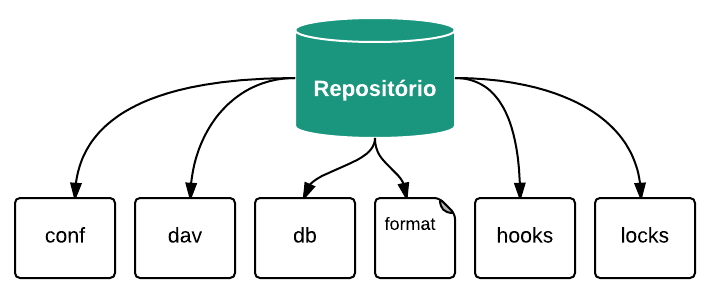
\includegraphics[scale=1]{figuras/repositorio.png}
\caption{Estrutura do repositório. Baseado em \cite{svn-book}}
\end{figure}


\begin{itemize}

\item conf: Pasta que contém arquivos de configuração do repositório.

\item dav: Pasta que contém arquivos utilizados pelo mod\_dav\_svn.

\item db: Pasta que armazena os dados versionados.

\item format: Arquivo que indica o número da versão do repositório.

\item hooks: Pasta que contém modelos de scripts

\item locks: Pasta para arquivos bloqueados, é utilizado no rastreamento dos acessos ao repositório.

\end{itemize}

\subsection{Disponibilizando um repositório}

\subsubsection{Escolhendo um servidor}

Um repositório pode ser mantido apenas localmente e seu acesso torna-se restrito à máquina a qual ele foi criado. Mas isso não é muito vantajoso, dessa forma um repositório deve ser disponbilizado em um servidor para que as pessoas possam acessá-lo de qualquer lugar. Dessa forma, \cite{svn-book} recomenda os servidores da Tabela \ref{tab:servidores}.

\begin{flushleft}
\begin{table}[!h]

\caption{Comparação entre os servidores. Fonte: \cite{svn-book}}
\label{tab:servidores}
\begin{tabular}{|l|l|l|l|}
\hline
\rowcolor[HTML]{01796F} 
{\color[HTML]{000000} \textbf{Característica}}                            & {\color[HTML]{000000} \textbf{\begin{tabular}[c]{@{}l@{}}Apache + \\ mod\_dav\_svn\end{tabular}}}                                                                           & {\color[HTML]{000000} \textbf{svnserve}}                                                                                                              & {\color[HTML]{000000} \textbf{\begin{tabular}[c]{@{}l@{}}svnserve\\ sobre SSH\end{tabular}}}                                       \\ \hline
\begin{tabular}[c]{@{}l@{}}Opções de \\ autenticação\end{tabular}         & \begin{tabular}[c]{@{}l@{}}Autenticação básica \\HTTP(S), certificados \\ X.509, LDAP,\\ NTLM, \\ou quaisquer \\ outros mecanismos \\disponíveis ao  \\ Apache httpd\end{tabular} & CRAM-MD5                                                                                                                                              & SSH                                                                                                                                \\ \hline
\begin{tabular}[c]{@{}l@{}}Opções para \\ contas de usuários\end{tabular} & \begin{tabular}[c]{@{}l@{}}arquivo 'users' \\ privativo\end{tabular}                                                                                                         & \begin{tabular}[c]{@{}l@{}}arquivo 'users' \\ privativo\end{tabular}                                                                                                           & contas no sistema                                                                                                                  \\ \hline
\begin{tabular}[c]{@{}l@{}}Opções de \\ autorização\end{tabular}          & \begin{tabular}[c]{@{}l@{}}acesso leitura/escrita pode \\ser dado para o \\repositório como um \\ todo, ou especificado por \\ caminho\end{tabular}                              & \begin{tabular}[c]{@{}l@{}}acesso leitura/escrita\\  pode ser dado para\\  o repositório como um\\  todo, ou especificado \\ por caminho\end{tabular} & \begin{tabular}[c]{@{}l@{}}acesso leitura/escrita\\  passível \\ de ser dado\\  apenas ao repositório\\  como um todo\end{tabular} \\ \hline
Criptografia                                                              & através de SSL opcional                                                                                                                                                     & nenhuma                                                                                                                                               & túnel SSH                                                                                                                          \\ \hline
Registro de log                                                           & \begin{tabular}[c]{@{}l@{}}logs completos \\do Apache para cada \\ requisição HTTP, \\ com opcional log\\  “alto nível” para operações\\ do cliente em geral\end{tabular}     & sem log                                                                                                                                               & sem log                                                                                                                            \\ \hline
Interoperabilidade                                                        & \begin{tabular}[c]{@{}l@{}}parcialmente usável por \\ outros clientes WebDAV\end{tabular}                                                                                   & \begin{tabular}[c]{@{}l@{}}se comunica apenas \\ com clientes svn\end{tabular}                                                                        & \begin{tabular}[c]{@{}l@{}}se comunica apenas\\  com clientes svn\end{tabular}                                                     \\ \hline
\begin{tabular}[c]{@{}l@{}}Visualização \\ pela web\end{tabular}          & \begin{tabular}[c]{@{}l@{}}suporte existente limitado,\\ ou também \\ por meio de ferramentas \\ de terceiros \\ como o ViewVC\end{tabular}                                      & \begin{tabular}[c]{@{}l@{}}apenas por meio de\\  ferramentas \\de terceiros \\ como o ViewVC\end{tabular}                                               & \begin{tabular}[c]{@{}l@{}}apenas por meio de \\ ferramentas \\de terceiros\\  como o ViewVC\end{tabular}                            \\ \hline
Velocidade                                                                & um pouco mais lento                                                                                                                                                         & \begin{tabular}[c]{@{}l@{}}um pouco mais \\ rápido\end{tabular}                                                                                       & \begin{tabular}[c]{@{}l@{}}um pouco \\ mais rápido\end{tabular}                                                                    \\ \hline
\begin{tabular}[c]{@{}l@{}}Configuração\\  inicial\end{tabular}           & um tanto complexa                                                                                                                                                           & extremamente simples                                                                                                                                  & \begin{tabular}[c]{@{}l@{}}Moderamente \\ simples\end{tabular}                                                                                                \\ \hline
\end{tabular}
\end{table}

\end{flushleft}

\subsubsection{Escolhendo um banco de dados}

\subsection{Acessando um repositório}

  Os repositórios criados para controle de versão com o SVN são acessados através de URLs, seguindo os seguintes padrões \cite{svn-book}:

\begin{centering}

\textbf{Para o servidor:} É especificado o nome do servidor e a porta.

\colorbox{PineGreen}{
\begin{minipage}{220px}
  \textbf{http://svn.example.com:9834/repos}
\end{minipage}
}

\textbf{Para repositórios locais:} a URL ganha o prefixo \textit{file:}. Podem ser escritos com o nome do servidor, ou sem.
\end{centering}

\begin{multicols}{2} 


\flushright{O nome do servidor como \textit{localhost}:

\colorbox{PineGreen}{
\begin{minipage}{210px}
  \textbf{file://localhost/caminho/repositorio}
\end{minipage}
}
}

Ou sem especificação do servidor:

\colorbox{PineGreen}{
\begin{minipage}{200px}
\flushleft{ 
  \textbf{file:///caminho/repositorio}
}
\end{minipage}
}

\end{multicols}

As possíveis URLs de acesso podem ser vistas na Tabela \ref{tab:urls}.

\begin{table}[!h]
\centering
\caption{URLs de acesso ao repositório. Fonte: \cite{svn-book}}
\label{tab:urls}
\begin{tabular}{|l|l|}
\hline
\rowcolor[HTML]{01796F} 
{\color[HTML]{000000} \textbf{Esquema}} & {\color[HTML]{000000} \textbf{Método de Acesso}}                             \\ \hline
file:///                                & acesso direto ao repositório (em um disco local).                            \\ \hline
http://                                 & acesso via protocolo WebDAV em um servidor Apache especialmente configurado. \\ \hline
https://                                & mesmo que http://, mas com encriptação SSL.                                  \\ \hline
svn://                                  & acesso via protocolo próprio em um servidor svnserve.                        \\ \hline
svn+ssh://                              & mesmo que svn://, mas através de um túnel SSH.                               \\ \hline
\end{tabular}
\end{table}



\subsection{Cópias de trabalho}
  
O SVN trabalha com cópias de trabalho. Uma cópia de trabalho consiste na mesma estrutura do repositório para uso privado. Ou seja, é a cópia local do repositório que pode ser editada pelo usuário. 

Para criar uma cópia de trabalho deve ser digitado o seguinte comando \cite{svn-book}:


\begin{centering}
\colorbox{PineGreen}{
\begin{minipage}{320px}
  \textbf{svn checkout http://svn.example.com:9834/repositorio}
\end{minipage}
}

\end{centering}

O repositório pode ser configurado com a estrutura de pastas que o usuário desejar, todavia existe um padrão recomendado que pode ser visto na Figura 
\ref{estrutura_repo}.

\begin{figure}[!htb]
\label{estrutura_repo}
\centering
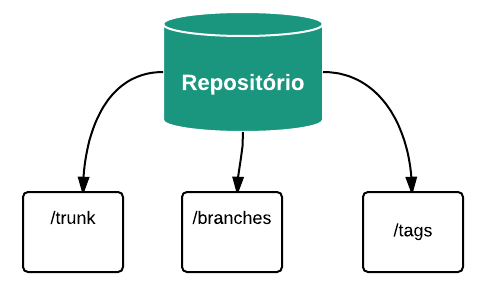
\includegraphics[scale=1]{figuras/estrutura_repo.png}
\caption{Estrutura recomendada do repositório. Baseado em \cite{svn-book}}
\end{figure}


\pagebreak

\subsection{Como funciona a relação entre o repositório e a cópia de trabalho?}

\begin{figure}[!htb]
\centering
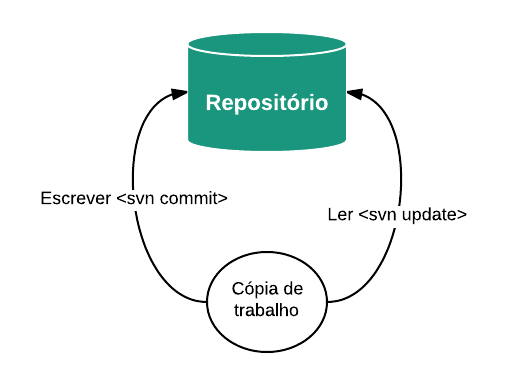
\includegraphics[scale=1]{figuras/repositorio_copia.png}
\caption{Comunicação entre cópia de trabalho e repositório. Baseado em \cite{svn-book}}
\end{figure}


Para que os outros membros do projeto tenham acesso ao que foi produzido na cópia de trabalho, o SVN permite que o usuário escreva no repositório as alterações feitas
e para ter acesso às atualizações feitas por outros membros, é permitido ao usuário ler o repositório \cite{svn-book}.

\begin{multicols}{2} 


\flushright{Para escrever}:{

\colorbox{PineGreen}{
\begin{minipage}{210px}
  \textbf{svn commit <nome do arquivo modificado> -m <"mensagem\">}
\end{minipage}
}
}

Para ler:

\colorbox{PineGreen}{
\begin{minipage}{200px}
\flushleft{ 
  \textbf{svn update}
}
\end{minipage}
}

\end{multicols}

\section{Passo a passo para o uso das principais funcionalidades da ferramenta}

Para ver os arquivos modificados o comando é: "svn status"

Para mostrar as diferenças m um arquivo "svn diff"

Para criar uma cópia de trabalho o comando é "svn checkout"

Para ver as revisões criadas o comando é: "svn status --verbose"

Para mostrar o histórico de mudanças o comando é "svn log"

Para desfazer as alterações em um arquivo: "svn revert <arquivo>"

Para criar uma branch, deve ser ser feita uma cópia da pasta trunk para a pasta de branchs com o seguinte comando:

"svn copy <caminho da pasta original> \ <caminho da pasta de destino, essa pasta deve possuir o nome da branch> -m "mensagem\">"

\section{Verificação das funcionalidades descritas a seguir em forma de pergunta:}

\begin{itemize}
  \item A ferramenta provê mecanismo de backup dos itens controlados pela ferramenta?

    Sim. O SVN provê um comando que possibilita a realização de um backup do repositório, caso algo dê errado. O comando é:
    "svnadmin hotcopy <caminho do repositorio> <caminho de backup>"

  \item A ferramenta provê algum mecanismo de controle de acesso?
    Sim. No arquivo "svnserve.conf" são descritos os níveis de acesso para usuários autenticados e não autenticados

  \item A ferramenta controla arquivos de diversos formatos, seja código, executáveis, documentação e diagramas?
    Sim. O SVN controla versão de todos os documentos colocados no repositório.

  \item A ferramenta registra versões dos itens de configuração?
    Sim. Cada alteração feita é registrada em um número de revisão. É possível visualizar um histórico de alterações com as seguintes informações:

    \subitem Nome do autor da alteração
    \subitem Data e hora
    \subitem Mensagem que descreve a alteração

  \item É possível visualizar as diferenças entre as versões incluindo a razão para estas 
  diferenças?
  O SVN permite a visualização das diferenças entre as versões, mas não apresenta a razão das diferenças.
  
  \item É possível identificar dependências entre artefatos, são elas: artefatos que pertencem a um mesmo item de configuração; itens de configuração de um componente; versão de itens de configuração de uma baseline; artefatos que são utilizados para construir um outro artefato  (por exemplo, um código é usado para construir a funcionalidade de um outro código)?
  
  
  \item É possível selecionar itens de configuração compatível com a versão válida e consistente do
  produto?
  \item É possível fazer snapshots ou congelar o estado de um produto a qualquer momento?
  \item A ferramenta provê mecanismos que facilitem a análise do impacto de se fazer uma mudança?
  \item É possível recuperar o histórico de todas as mudanças realizadas no itens controlados pela
  ferramenta?
  \item É possível recuperar o log de todos os detalhes do trabalho realizado?
  \item A ferramenta provê mecanismos para registrar estatísticas?
  \item A ferramenta provê mecanismos para examinar estado dos itens?
  \item A ferramenta provê mecanismos para selecionar aspectos para os quais deseja-se gerar relatório
  de acompanhamento de estado de configuração e gerar tal relatório?
  \item A ferramenta adverte sobre acesso inadequado a qualquer item para evitar mudanças não justificadas
  ou conflitos de mudanças?
  \item A ferramenta provê meios para monitorar bugs (quem, como e quando o bug foi gerado)?
  \item A ferramenta provê meios que facilitem a propagação de mudanças de maneira controlada
  através de diferentes versões de itens?
  \item A ferramenta provê mecanismos para facilitar a comunicação entre os interessados nos itens de
  configuração controlados?
  \item A ferramenta provê mecanismos para resolução de conflitos quando for necessário fazer merge
  de mudanças?
  Sim. O SVN usa o modelo \textit{copy-modify-merge}(copiar-modificar-fundir) que adverte aos usuários quando sua cópia local está em situação de conflito.
  Esse modelo funciona da seguinte maneira: 
  Cada usuário cria uma cópia de trabalho pessoal a partir do repositório do projeto. Os usuários, então, 
  trabalham de forma simultânea e independente fazendo modificações em suas cópias privadas. Quando as mudanças 
  feitas nas cópias privadas são submetidas a uma nova versão ao repositório do projeto, o SVN então vai fundir essas cópias.
  Quando Dois usuários fazem alteração a uma cópia ao mesmo tempo e submete a uma nova versão, o último usuário que submeter será informado
  que a sua cópia privada está desatualizada, ou seja, o arquivo de seu repositório local foi alterado desde a 
  última vez em que ele foi copiado. Com isso, o SVN pode ajudá-lo a fundir todas as alterações do repositório na sua cópia. 
  O SVN não consegue solucionar possíveis conflitos automaticamente, mas ele sinaliza no arquivo as alterações que estão em conflito
   permitindo com que o usuário resolva manualmente.
\end{itemize}
